\section{Problem}

For our CS598PS project, we entered a Kaggle competition that requires us to
identify mobile devices from accelerometer data~\cite{Kaggle2013}. Since
everyone moves differently and that most devices are being equipped with
accelerometers nowadays, the purpose of this competition is to investigate the
feasibility of deanonymizing users of mobile device from their accelerometer
data using machine learning techniques.

In the competition, approximately 60 million unique samples of accelerometer
data are collected from 387 different devices. These are split into equal sets
for training and test. Samples in the training set are labeled with the unique
device from which the data was collected. The test set is demarcated into 90k
sequences of consecutive samples from one device.

\begin{figure}
  \centering
  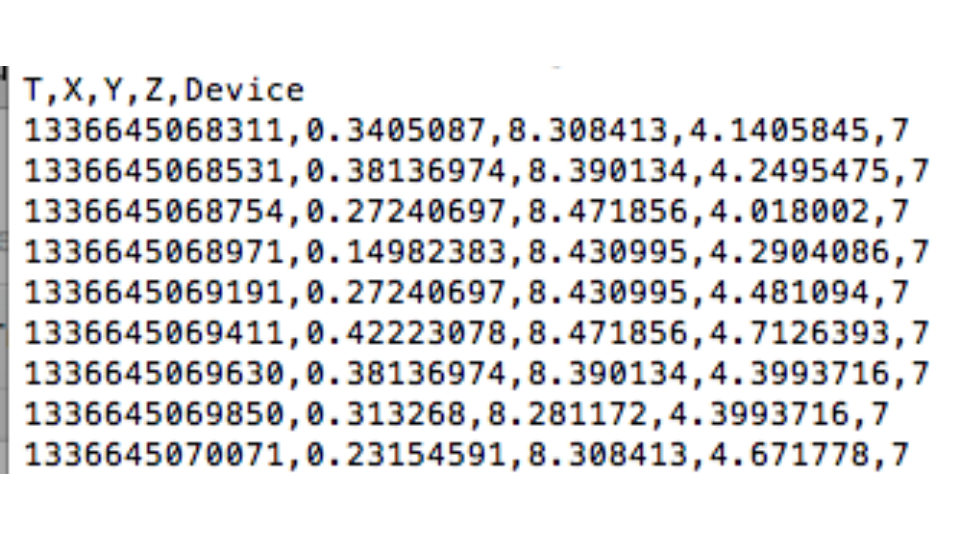
\includegraphics[width=\linewidth]{./figs/train_data.png}
  \caption{Format of training data.}
  \label{fig:train}
\end{figure}

\begin{figure}
  \centering
  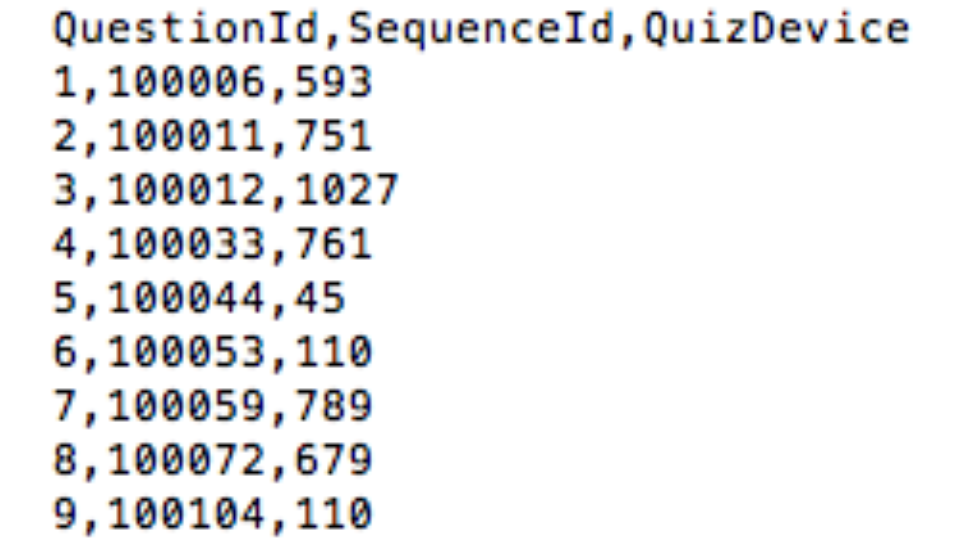
\includegraphics[width=\linewidth]{./figs/questions.png}
  \caption{Format of question data.}
  \label{fig:question}
\end{figure}

We are given two datasets mainly. The first dataset is the training data as
indicated in Figure~\ref{fig:train}. In this file, the format is that the first
field contains the timestamp, T, in which the data is being taken while the
next three fields indicate the coordinates of the accelerometer; X, Y, Z. The
last field contains the DeviceId which indicates the unique id of the device
that generated this particular data point. The second dataset is the question
data as indicated in Figure~\ref{fig:question}. In this file, the first field
is the id of the question, QuestionId, the second field is unique number
assigned to each sequence of sample, SequenceId, and the third field is the
professed device id that generated the sequence of accelerometer data that we
need to either agree or disagree to.
